\documentclass[preprint,12pt]{aastex}

\def\mearth{{\rm\,M_\oplus}}
\def\rearth{{\rm\,R_\oplus}}
\def\msun{{\rm\,M_\odot}}
\def\rsun{{\rm\,R_\odot}}
\def\lsun{{\rm\,L_\odot}}
\def\gsim{~\rlap{$>$}{\lower 1.0ex\hbox{$\sim$}}}
\def\lsim{~\rlap{$<$}{\lower 1.0ex\hbox{$\sim$}}}
\def\etal{{\it et al.\thinspace}}
\def\wpmsq{W m$^{-2}$}
\def\etal{{\it et al.\thinspace}}
\def\eg{{\it e.g.\ }}
\def\etc{{\it etc.\ }}
\def\ie{{\it i.e.\ }}
\def\cf{{\it c.f.\ }}
\def\acen{{$\alpha$~Cen}}

\def\tess{{\it TESS}}
\def\kepler{{\it Kepler}}
\def\jwst{{\it JWST}}

\def\vplanet{\texttt{\footnotesize{VPLANET}}}
\def\atmesc{\texttt{\footnotesize{ATMESC}}}
\def\distorb{\texttt{\footnotesize{DISTORB}}}
\def\distrot{\texttt{\footnotesize{DISTROT}}}
\def\eqtide{\texttt{\footnotesize{EQTIDE}}}
\def\poise{\texttt{\footnotesize{POISE}}}
\def\radheat{\texttt{\footnotesize{RADHEAT}}}
\def\thermint{\texttt{\footnotesize{THERMINT}}}
\def\stellar{\texttt{\footnotesize{STELLAR}}}
\def\galhabit{\texttt{\footnotesize{GALHABIT}}}

\bibliographystyle{apj}
\usepackage{multicol}

\begin{document}

\title{The Habitability of Proxima Centauri b I: Environmental Context}
\author{Rory Barnes\altaffilmark{1,2,3}, Russell Deitrick\altaffilmark{1,2}, Rodrigo Luger\altaffilmark{1,2}, Peter E. Driscoll\altaffilmark{4,2}, Thomas R. Quinn\altaffilmark{1,2}, David P. Fleming\altaffilmark{1}, Benjamin Guyer, Diego V. McDonald, Victoria S. Meadows, Giada Arney, David Crisp, Shawn D. Domagal-Goldman, Andrew Lincowski, Jacob Lustig-Yaeger, Eddie Schwieterman}
\altaffiltext{1}{Astronomy Department, University of Washington, Box 951580, Seattle, WA 98195}
\altaffiltext{2}{NASA Astrobiology Institute -- Virtual Planetary Laboratory Lead Team, USA}
\altaffiltext{3}{E-mail: rory@astro.washington.edu}

\begin{abstract}
\end{abstract}

\section{Introduction\label{sec:intro}}

The discovery of Proxima Centauri b, hereafter Proxima b, heralds a
new era in the exploration of exoplanets. Although very little is
currently known about it and its environment, the planet is likely
terrestrial and receives an incident flux that places it in the
``habitable zone'' (HZ)
\citep{Kasting93,Selsis07,Kopparapu13}. Moreover, Proxima b is
distinct from other discoveries in that it is the first potentially
habitable planet that could be directly characterized by space
telescopes such as WFIRST and concept missions such as LUVOIR, HDST,
and HabEx. Such remote sensing is possible because the angular
separation of the planet and star as viewed from Earth is
37 mas. Proxima b will likely be the first exoplanet to be
spectroscopically probed for active biology.

The interpretation of these spectra require a firm understanding of
the history of Proxima b and its host system. Proxima b exists in an
environment that is significantly different from Earth and has likely
experienced different phenomena that could preclude or promote the
development of life. When viewed across interstellar distances,
biology is best understood as a planetary process; life is a global
phenomenon that alters geochemical and photochemical
processes. Spectroscopic indicators of life, \ie biosignatures, can
only be identified if the abiotic processes on a planet are understood
-- no single feature in a spectrum is a ``smoking gun'' for life on
all planets. A robust detection of extraterrestrial life requires that
all plausible non-biological sources for an observed spectral
features can be ruled out. This requirement is a tall order,
especially in light of the expected diversity of terrestrial
exoplanets in the galaxy, but Proxima b may offer the best opportunity
to begin the scientific process of searching for unambiguous signs of
life.

In this study we leverage the known (but sparse) data on Proxima b and
its host system to predict the range of evolutionary pathways that the
planet may have experienced. As we show below, many histories are
possible and depend on factors ranging from the cooling rate of b's
core to the orbital evolution of the stellar system through the Milky
Way, and everywhere in between. The evolution of Proxima b, and by
extension its potential habitability, depends on physical processes
that have tended to be studied by scientists that work in different
fields, such as geophysics and astrophysics. However, for the purpose
of interpreting Proxima b, these divisions must be dismantled. Our
examination of Proxima b will draw on simple, but realistic, models
that have been developed in the fields of geophysics, planetary
science, atmospheric science and astrophysics. From this synthesis, we
identify numerous obstacles and opportunities for life to develop on
Proxima b, as well as lay a foundation for the future interpretation
of spectroscopic observations.

This paper is organized as follows. In $\S$~\ref{sec:obs} we review
the observational data on the system and the immediate implications
for habitability. In $\S$~\ref{sec:models} we describe models to
simulate the evolution of the system, with a focus on habitability. In
this section we introduce a new software package called \vplanet,
which couples physical models of planetary interiors, atmospheres,
spins and orbits, stellar evolution, and galactic effects. In
$\S$~\ref{sec:results} we present results of these models. An
exhaustive analysis of all histories is too large to present here, so
in this section we present highlights and end-member cases that
bracket the plausible ranges. In $\S$~\ref{sec:disc} we discuss the
results and identify additional observations that could improve
modeling efforts and connect our results to the companion paper
\citep{Meadows16}. Finally in $\S$~\ref{sec:concl} we draw our
conclusions.

\section{Observational Constraints \label{sec:obs}}

In this section we review what is known about the triple star system
Alpha Centauri (hereafter \acen) of which Proxima Centauri may be a
member. This star system has been studied carefully for centuries as
it is the closest to Earth. We will first review the direct
observational data, then we will make whatever inferences are possible
from those data, and finally we qualitatively consider how these data
constrain the possibility for life to exist on Proxima b, which will
then guide the models described in the next section.

\subsection{Properties of the Proxima Planetary System}

Precious little data exist for Proxima b. The radial velocity data
reveal a planet with a minimum mass $m$ of 1.27~$\mearth$, an orbital period $P$
of 11.186 days, and an orbital eccentricity $e$ less than 0.35 and
\cite{AngladaEscude16} report a mean longitude $\lambda$ of $110^\circ$. These
data are the extent of the direct observational data on the planet,
but even the minimum mass relies on uncertain estimates of the mass of
the host star, described below.

Proxima b may not be the only planet orbiting Proxima
Centauri. The Doppler data suggest the presence of another planetary
mass companion with an orbital period near 215 days, but it is not
definitive yet \citep{AngladaEscude16}. If present, the planet has a
projected mass of $\lesssim~10~\mearth$, consistent with previous
non-detections \citep{EndlKurster08,Barnes14,Lurie14}. The orbital
eccentricity and it relative inclination to Proxima b's orbit are also
unknown, but as described below, could take any value that permits
dynamical stability. Additional, lower mass and/or more distant,
planetary companions could also be present in the system.

\subsection{Properties of the Host Star}

As Proxima Centauri is the closest star to Earth, it has been studied
extensively since its discovery 100 years ago \citep{Innes1915}.  It
has a radius $R_*$ of $0.14~\rsun$, a temperature $T_{eff}$ of 3050 K, a
luminosity $L_*$ of $0.00155~\lsun$~\citep{Boyajian12}, and a rotation
period $P_*$ of 83 days \citep{Benedict98}. \cite{Wood01} searched for
evidence of stellar winds, but found none, indicating mass loss rates
$\dot{M}_*$ less than 20\% of our Sun's, \ie
$<4~\times~10^{-15}~\msun/\textrm{yr}$. Proxima Centauri possesses a
much larger magnetic field ($B~=~600~\pm~150$~G) than our Sun (1 G)
\citep{ReinersBasri08}, but somewhat low compared to the majority of
low mass stars.

Like our Sun, Proxima Centauri's luminosity varies slowly with time
due to starspots \citep{Benedict93}. HST observations of Proxima
Centauri found variations up to 70 mmag in $V$ \citep{Benedict98},
which, corresponds to about a 17.5\% change with a period of 83.5 days
(\ie the rotation period). Moreover, \citep{Benedict98} found evidence
for two discrete modes of variability, one lower amplitude mode
($\Delta~V~\sim~30$~mmag) with a period of $\sim 42$ days, and a
larger amplitude mode ($\Delta~V~\sim~60$~mmag with a period of 83
days. These periods are a factor of 2 of each other, leading
\cite{Benedict98} to suggest that sometimes a large spot (or cluster
of spots) is present on one hemisphere only, while at other times
smaller spots exist on opposite hemispheres. Regardless, incident
stellar radiation (``instellation'') variations of 17\% could impact
atmospheric evolution and surface conditions of a planet (the sun's
variation is of order 0.1\% \citep{Willson81}).

Additionally the magnetic field strength may vary with
time. \cite{Cincunegui07} monitored the H and K CaII lines, which are
indicators of chromospheric activity, as well as H$\alpha$ for 7 years
and found modest evidence for a 442 day cycle in stellar
activity. Although it is unclear the strength of Proxima's magnetic
field at the orbit of planet b, it could contribute to the stability
of b's atmosphere and potentially affect any putative life on b.

Proxima Centauri is a known flare star
\citep{Shapley51}\footnote{Although Shapley is the sole author of his
  1951 manuscript, the bulk of the work was performed by two female
  assistants, C.D. Boyd, and V.M. Nail.}  and indeed several flares
were reported during the Pale Red Dot campaign
\cite{AngladaEscude16}. \cite{Walker81} performed the first study of
the frequency of flares as a function of energy, finding that high
energy events ($\sim~10^{30}$ erg) occurred about once per day, while
lower energy events ($\sim~10^{28}$ erg) occurred about once per
hour. Numerous observational campaigns since then have continued to
find flaring at about this frequency
\citep{Benedict98,AngladaEscude16}.

\subsection{Properties of the Stellar System}

Proxima Centauri is $\approx~15,000$ AU from two larger stars, Alpha
Centauri A and B (hereafter \acen~A and B), but all three have the
same motion through the galaxy. Finally, the proper motion and radial
velocity of the center of mass of \acen~A and B permit the calculation
of the system's velocity relative to the local standard of
rest. \cite{Poveda96} find the three velocities are ($U,V,W$) =
(-25,-2,13) km/s for the center of mass. This velocity implies the
system is currently approaching Earth, and is on a roughly circular
orbit around the galaxy with an eccentricity of 0.07
\cite{AllenHerrera98}.

A recent, careful analysis of astrometric and HARPS RV data by
\cite{PourbaixBoffin16} found the masses of the two stars to be 1.133
and $0.972~\msun$, respectively, with an orbital eccentricity of 0.52
and a period of 79.91 years. The similarities between both A and B and
the Sun, as well as their low apparent magnitudes, has allowed
detailed studies of their spectral and photometric properties. These
two stars (as well as Proxima) form a foundation in stellar astrophysics,
and hence a great deal is known about A and B. However, as we describe
below, many uncertainties still remain regarding these two stars.

The spectra of \acen~A and B can provide information about the stars
temperature, gravitational acceleration in the photosphere, rotation
rate, and composition. That these features can be measured turns out
to be critical for our analysis of the evolution of Proxima b. Proxima
Centauri is a low mass star and hence its composition is far more
difficult to measure than for G and K dwarfs like \acen~ A and
B. Recently, \cite{HinkelKane13} completed a reanalysis of published
compositional studies, rejecting the studies of \citep{Laird85} and
\citep{NeuforgeMagain97} because they were too different from the
other 5 they considered, and found the means of metallicities [Fe/H]
of the two stars to be +0.28 and +0.31 and with a large spread of 0.16
and 0.11, respectively. While it is frustrating that different groups
have arrived at significantly different iron abundances, it is certain
the stars are more metal-rich than the Sun. 

\citep{HinkelKane13} go on to examine 21 other elements, including C,
O, Mg, Al, Si, Ca, and Eu. These elements can be important for the
bulk composition and/or are tracers of other species that are relevant
to planetary processes. In nearly all cases, the relative abundance of
these elements to Fe is statistically indistinguishable from the solar
ratios. Exceptions are Na, Zn and Eu in \acen~A, and V, Zn, Ba
and Nd in \acen~B. The discrepancies between the two stars is
somewhat surprising given their likely birth from the same molecular
cloud. On the other hand, the high eccentricity of their orbit could
point toward a capture during the open cluster phase (cite). For all
elements beside Eu, the elemental abundances relative to Fe are larger
than in the Sun. In particular, it seems likely that the stars are
significantly enriched in Zn.

\acen~A and B are large enough and bright enough for asteroseismic
studies that can reveal physical properties and ages of stars to a few
percent, for high enough quality data (cite). Indeed, these two stars
are central to the field of asteroseismology, and have been studied in
exquisite detail. However, significant uncertainties persist in our
understanding of these stars, despite all the observational
advantages.

A recent study undertook a comprehensive Bayesian analysis of \acen~A
with priors on radius, composition, and mass derived from
interferometric, spectroscopic and astrometric measurements,
respectively \citep{Bazot16}. Their adopted metallicity constraint
comes from \citep{NeuforgeMagain97} via \citep{Thoul03}, which was
rejected by the \citep{HinkelKane13} analysis. They also used an older
mass measurement from \citep{Pourbaix02}, which is slightly smaller
than the updated mass from \citep{PourbaixBoffin16}. They then used an
asteroseismic code to determine the physical characteristics of
A. Although the mass of A is similar to the Sun at $1.1~\msun$, the
simulations of Bazot et al., found that \acen~A's core lies at the
radiative/convective boundary and the transition between pp- and
CNO-dominated energy production chains in the core. Previous results
found the age of \acen~A to be 4.85 Gyr with a convective core
\citep{Thevenin02}, or 6.41 Gyr without a convective core
\citep{Thoul03}. The ambiguity is further increased by uncertainty in
the efficiency of the $^{14}$N(p,$\gamma$)$^{15}$O reaction rate in
the CNO cycle, and by uncertainty regarding the possibility of
convective overshooting of hydrogen into the core. They also consider
the role of ``microscopic diffusion'' which is the settling heavy
elements over long time intervals. All these uncertainties
prevent a precise and accurate measurement of \acen~A's
age. Combining the different model predictions and include 1$\sigma$
uncertainties, the age of \acen~A is between 3.4 and 5.9 Gyr,
with a mean of 4.78 Gyr.

\acen~B has also been studied via asteroseismology, but as with A, the
results have not been consistent. \cite{Lundkvist14} find significant
discrepancies between their ``Asteroseismology Made Easy'' age (1.5
Gyr) with other values, but with uncertainties in excess of 4 Gyr. The
asteroseismic oscillations on B are much smaller than on A, which make
analyses more difficult \citep[see, \eg][]{CarrierBourban03},
leading to the large uncertainty. Combining studies of A and B, we
must conclude that the ages of the two stars are uncertain to at least
25\%. Given the difficulty in measuring B's asteroseismic pulsations,
we will rely on A's asteroseismic data and assume the age of A and B
to be $4.8^{+1.1}_{-1.4}$.

\subsection{Inferences from the Observational Data}

Because Proxima b was discovered indirectly, its properties and
evolution depend critically on our knowledge of the host star's
properties. Although many properties are known, the mass $M_{Prox}$,
age, $T$, and composition are not. The spectra and luminosity suggest
the mass of Proxima is $\sim~0.12~\msun$ \citep{Delfosse00}. If we
adopt this value, then the semi-major axis of b's orbit is 0.0485~AU
and the planet received 65\% of the instellation as Earth receives
from the Sun \cite{AngladaEscude16}.  Note that \cite{Sahu14}
suggested that Proxima's proper motion sent it close enough to two
background stars for the general relativistic deflection of their
light by Proxima to be detectable with HST and should allow the determination of
$M_{Prox}$ to better than 10\%, but those results are not available
yet.

Additional inferences rely on the assumption that Proxima formed with
the \acen~binary.  The similarities in the proper motion and parallax
between Proxima and \acen~immediately led to speculation as to whether
the stars are ``physically connected or members of the same drift''
\citep{Voute1917}, \ie are they bound or members of a moving group?
The intervening century has failed to resolve this central
question. If Proxima is just a random star in the solar neighborhood,
\cite{MatthewsGilmore93} concluded that probability that Proxima would
appear so close to \acen~is about 1 in a million, suggesting it is
very likely the stars are somehow associated with each other. Using
updated kinematic information, \citep{Anosova94} conclude that Proxima
is not bound, but instead part of a moving group consisting of about a
dozen stellar systems. \cite{WertheimerLaughlin06}'s reanalysis found
that the observational data favor a configuration that is at the
boundary between bound and unbound orbits. However, their best fit
bound orbit is implausibly large as the semi-major axis is 1.31 pc,
\ie larger than the distance from Earth to
Proxima. \cite{MatvienkoOrlov14} also failed to unequivocally resolve
the issue, and conclude that RV precision of better than 20 m/s is
required to determine if Proxima is bound, which should be available
in the data from \citep{AngladaEscude16}. Perhaps the discovery data
for Proxima b will also resolve this long-standing questions.

Regardless of whether Proxima is bound or not, the very low
probability that the stars would be so close to each other strongly
supports the hypothesis that the stars formed in the same star
cluster. We will assume that they are associated and have
approximately equal ages and similar compositions. An age near 5 Gyr
for Proxima is also consistent with its rotation period and relatively
modest activity levels and magnetic field \citep{ReinersBasri08}.

Planet formation around M dwarfs is still relatively understudied, but
it must proceed in a qualitatively similar way as for Sun-like stars,
\ie the planet form from a disk of dust and gas. Relatively few
obserations of disks of M dwarfs exist
\citep[\eg][]{Hernandez07,WilliamsCieza11,Luhman12,Downes15}, but
these data seem to point to a wide range of lifetimes for the gaseous
disks of 1--15~Myr. For Proxima the lifetime of the protoplanetary
disk is unknown, and could have been altered by the presence of
\acen~A and B, so any formation pathway or evolutionay process
permitted within this constraint is plausible.

The radial velocity data combined with $M_{Prox}$ only provide a
minimum mass, but significantly larger planet masses are unlikely
geometrically, and very large masses can be excluded because they
would incite detectable astrometric signals (note that the minimum
mass solution predicts an astrometric orbit of the star of $\sim$1
microsecond of arc). It is very likely the planet has a mass less than
10~$\mearth$, and probably $<~3~\mearth$. We will assume the latter
possibility is true, and hence the planet is likely rocky, based on
statistical inferences of the population of \kepler~planets
\cite{WeissMarcy14,Rogers15}. However, even at the minimum mass, we
cannot exclude the possibility that Proxima b possesses a significant
hydrogen envelope. Such a world is unlikely to be habitable \citep[but
  see][]{PierrehumbertGaidos11} and hence we cannot at this time state
unequivocally that Proxima b is not a ``mini-Neptune'', let alone if
it is habitable.

If non-gaseous, the composition is still highly uncertain and depends
on the unknown formation process. Several possibilities exist
according to recent theoretical studies: 1) the planet formed {\it in
  situ} from local material; 2) the planet formed at a larger
semi-major axis and migrated in while Proxima still possessed a
protoplanetary disk; or 3) an instability in the system occurred that
impulsively changed b's orbit. For case 1, the planet may be depleted
in volatile material \citep{Raymond07,Lissauer07}, but could still
possess a significant water inventory \citep{Mulders15}. For case 2,
the planet would have likely formed beyond the snowline and hence
could be very water-rich \citep{CarterBond12}. For case 3, the planet
could be either volatile-rich or poor depending on its initial
formation location as well as the details of the instability, such as
the frequency of impacts that occurred in its aftermath. We conclude
that all options are possible given the data and for simplicity will
assume the planet is Earth-like in composition. If we adopt the
silicate planet scaling law of \cite{Sotin07}, the radius of a
$1.3~\mearth$ planet is $1.07~\rearth$.

\subsection{Implications for Proxima b's Evolution and Habitability}

Given the above observations and their immediate implications, this
planet may be able to support life. All life on Earth requires three
basic ingredients: Water, energy, and the bioessential elements of C,
H, O, N, S and P. Additionally these ingredients must be present in an
environment that is stable in terms of temperature, pressure and pH
for long periods of time. As we describe in this subsection, these
properties are possible on Proxima b and hence the planet is
potentially habitable, defined here to mean liquid water persisting on
the surface for long timescales.

Proxima's luminosity and effective temperature combined with b's
orbital semi-major axis place the planet in the habitable zone (HZ) of
Proxima and nearly in the same relative position of Earth in the Sun's
HZ. More specifically, the planet receives about 65\% of Earth's
instellation, which places b in the ``optimistic'' HZ, meaning that it
would be very likely if the modern Earth would likely be habitable if
it received that instellation. Even allowing for observational
uncertainties, \cite{AngladaEscude16} find that the planet is in this
optimistic HZ.

However, its habitability depends on many more factors than just the
instellation. The planet must form with water and physical processes
cannot subsequently remove it. Additionally, even if water is present,
the evolution of Proxima depends on many other factors involving
stellar effects, the planet's internal properties, and the
gravitational influence of the other members of the stellar system.

The host star is about 10 times smaller and less massive than the Sun,
the temperature is about half that of the Sun, and the luminosity is
just 0.1\% that of the Sun. These differences are significant and can
have a profound effect on the evolution of Proxima b. Low mass stars
can take billions of years to begin fusing hydrogen into helium in
their cores, and the star's luminosity can change during that
time. Specifically, the star contracts at constant temperature and so
the star's luminosity drops with time. For the case of Proxima, this
stage lasted $\sim~1$~Gyr \cite{Baraffe15} and hence Proxima b
could have spend significant time interior to the HZ, \ie in a runaway
greenhouse state like Venus. This ``pre-main sequence'' phase could
either strip away a primordial hydrogen atmosphere to reveal a
``habitable evaporated core'' \citep{Luger15}, or, if b formed as a
terrestrial planet, it could desiccate that planet and build up an
oxygen-dominated atmosphere \citep{LugerBarnes15}. Thus, the large
early luminosity of the star could either be a help or hindrance for
b's habitability.

Low mass stars also show significant activity, \ie flares, coronal
mass ejections, and bursts of high energy radiation
\citep[\eg][]{West08}. This activity can change the composition of the
atmosphere through photochemistry, or even completely strip the
atmosphere away. The tight orbit of Proxima b places it at risk of
atmospheric stripping by these phenomena. A planetary magnetic field
could increase the probability of atmospheric retention by deflecting
charged particles, or it could decrease it by funneling high energy
particles into the magnetic poles and providing enough energy to
atmospheric particles to achieve escape velocity. Either way, the
frequency of flaring and other high energy events, as well as the
likelihood that Proxima b possesses a magnetic field, would be
invaluable in assessing the longevity of Proxima b's atmosphere.

The close-in orbit also introduces the possibility that tidal effects
can be significant on the planet. Tides can affect the planet in five
ways. First, they could cause the rotation rate to evolve to a
frequency that is equal to or similar to the orbital frequency, a
process typically called tidal locking
\citep{Dole64,Kasting93,Barnes16}. Second, they can drive the planet's
obliquity $\psi$ to zero or $\pi$ such that the planet has no seasons
\citep{Heller11}. Third, they can cause the orbital eccentricity to
change, usually (but not always) driving the orbit toward a circular
shape \citep{Darwin1880}. Fourth, they can cause frictional heating in
the interior called tidal heating
\citep{Peale79,Jackson08c,Barnes13}. Finally, the can cause the
semi-major axis to decay as orbital energy is transformed into
frictional heat \citep{Darwin1880,Barnes08}. Except in extreme cases,
these processes are unlikely to sterilize a planet, but they can
profoundly affect the planet's evolution.

Tidal locking many many researchers to conclude that planets of M
dwarfs are unlikely to support life because the atmospheres would
freeze out on the dark side \citep{Kasting93}. However, numerous
follow-up calculations have shown that tidal locking is not likely to
result in uninhabitable planets
\citep{Joshi97,Pierrehumbert11,Wordsworth11,Yang13,Shields16}. These
models all find that winds are able to transport heat to the back side
of the planet for atmospheres larger than about 0.3 bars. In fact,
synchronous rotation may actually allow habitable planets to exist
closer to the host star because cloud coverage develops at the
sub-stellar point and increases the planetary abledo
\citep{Yang13}. Thus, tidal locking may increase a planet's potential
to support life.

Although the abundances of elements relative to iron in \acen~A and B,
and by extension Proxima, are similar to the Sun's, there is no
guarantee that the abundance pattern is matched inside Proxima
b. Planet formation is often a stochastic process and composition
depends on the impact history of a given world. The planet could have
formed near its current location, which would have been relatively hot
early on and the planet could be relatively depleted in volatiles
\citep{Raymond07,Mulders15}. These studies may even overestimate
volatile abundances as they ignored the high luminosities that late M
dwarfs have during planet formation. Alternatively the planet could
have formed beyond the snowline and migrated in either while the gas
disk was still present, or later during a large scale dynamical
instability (see below). In those cases, the planet could be
volatile-rich.

The depletion of Eu in \acen~A is also of note as it is often a tracer
of radioactive material like $^{232}$Th and $^{238}$U
\citep{Young14}. These isotopes are primary drivers of the internal
energy of Earth, and hence if they are depleted in Proxima b, it
internal evolution could be markedly different than Earth's. However,
since no depletion is observed in \acen~B, it is far from clear that
such a depletion exists. One interesting radiogenic possibility is
that the planet could form sufficiently quickly ($\sim~1$~Myr) that
$^{26}Al$ could still provide energy to the planet's interior. Hence any
simulation of b's evolution should also consider its role.

The presence of additional planets can change the orbit and obliquity
of planet b through gravitational perturbations. These interactions
can change the orbital angular momentum of b and drive oscillations in
$e$, the inclination $i$, longitude of periastron $\varpi$, and
longitude of ascending node $\Omega$. Changes in inclination can lead
to changes in $\psi$ as the planet's rotational axis is likely fixed
in inertial space while the orbital plane precesses. These variations
can significantly affect climate evolution and possibly even the
planet's potential to support life \citep{Armstrong14}.

If Proxima is bound to \acen~A and B, then perturbations by passing
stars and torques by the galactic tide can cause drifts in Proxima's
orbit about A and B \citep{Kaib13}. During epochs of high
eccentricity, Proxima may swoop so close to A and B that their gravity
is able disrupt Proxima's planetary system. This could have occurred
at any time in Proxima's past and can lead to a total rearrangement of
the system. Thus, should additional planets exist in the Proxima
planetary system, could be present on almost any orbit, with large
eccentricities and large mutual inclinations with b's orbital plane.

The metallicity of Proxima Centauri is quite high for the solar
neighborhood, which has a mean of -0.11 and standard deviation of 0.18
\citep{AllendePrieto04}. Indeed, recent simulations of stellar
metallicity distributions in the galaxy find that at the sun's
galactic radius $R_{gal}$ of $\sim$8 kpc, stars cannot form with
[Fe/H]$ > +0.15$ \citep{Loebman16}. The discrepancy can be resolved by
invoking radial migration \citep{SellwoodBinney02} in which stars on
nearly circular orbits are able to ride corotation resonances with
spiral arms inward and outward. \cite{Loebman16} find that with
migration, the metallicity distribution of stars in the Sloan Digital
Sky Survey III's Apache Point Observatory Galactic Evolution
Experiment \citep{Hayden15} is reproduced.  Furthermore, Loebman et
al.\ find that stars in the solar neighborhood with [Fe/H] $> +0.25$
must have formed at $R_{gal} < 4.5$~kpc. We conclude that this system
has migrated outward at least 3.5~kpc, probably more. As the surface
density scale length of the galaxy is $\sim$2.5 kpc, this implies that
the density of stars at their formation radius was at least 5 times
higher than the solar radius.

The observed and inferred constraints for the evolution of Proxima b
are numerous, but the plausible range of evolutionary pathways is
diverse. The proximity of two solar-type stars complicates the
dynamics, but allows the extension of their properties to Proxima
Centauri. In the next sections we apply quantitative models of the
processes described in this section to full stellar system in order to
explore the possible histories of Proxima b in detail.

% Still to explore: Eu->Radiogenic, lifetimes of M dwarf disks, GCMs of tidally-locked planets 

\section{Models\label{sec:models}}

In this section we describe the models we use to consider the
evolution and potential habitability of Proxima b. We generally use
published models that are common to different disciplines of
science. Although the models come from disparate sources, we have
compiled them all into a new software program called \vplanet. This
code is designed to simulate exoplanet evolution, with a focus on
habitability. The problem of habitability is interdisciplinary, but we
find it convenient to break the problem down into more manageable
chunks, which we call ``modules,'' that are applied when
applicable. At this time, \vplanet~consists of simple models that are
all representable as an ordinary differential equation. Below we
describe qualitatively the modules and direct the reader to the
references for a quantitative description. We then briefly describe
how \vplanet~unifies these modules and integrates the system forward.

\subsection{Stellar Evolution: \stellar}
% Rodrigo

\subsection{Atmospheric Escape: \atmesc}
% Rodrigo

\subsection{Tidal Evolution: \eqtide}
% Rory
To model the tidal evolution of the Proxima system, we will use a
simple, but commonly-used model called the ``constant-phase-lag''
model \citep{Goldreich66,Greenberg09,Heller11}. This model reduces the
evolution to a single parameter $Q$ which sets the timescale for the
tidal evolution. While this model has known shortcoming
\citep{ToumaWisdom94,EfroimskyMakarov13}, it provides a qualitatively
accurate picture of tidal evolution, and is the model \cite{Kasting93}
used to calculate the ``tidal lock radius''. For this study, we use
the model described in \citep{Heller11}.

\subsection{Orbital Evolution: \distorb}
% Russell

\subsection{Rotational Evolution from Orbits and the Stellar Torque: \distrot}
% Russell

\subsection{Radiogenic Heating: \radheat}
% Peter

\subsection{Geophyiscal Evolution: \thermint}
% Peter

\subsection{Atmospheric Escape: \atmesc}
% Rodrigo

\subsection{Tidal Evolution: \eqtide}
% Rory
To model the tidal evolution of the Proxima system, we will use a
simple, but commonly-used model called the ``constant-phase-lag''
model \citep{Goldreich66,Greenberg09,Heller11}. This model reduces the
evolution to a single parameter $Q$ which sets the timescale for the
tidal evolution. While this model has known shortcoming
\citep{ToumaWisdom94,EfroimskyMakarov13}, it provides a qualitatively
accurate picture of tidal evolution, and is the model \cite{Kasting93}
used to calculate the ``tidal lock radius''. For this study, we use
the model described in \citep{Heller11}.

\subsection{Galactic Effects: \galhabit}
% Russell/Tom

\subsection{The Coupled Model: \vplanet}
% Rory
The previous modules are combined into a single software program
called \vplanet. This code is written in C and is designed to be
modular so that for any given body, only specific modules are applied
and specific parameters integrated forward. Parameters are integrated
using a 4th order Runge-Kutta scheme with a timestep equal to $\eta$
times the shortest timescale for all active parameters, \ie
$x/(dx/dt)$ where $x$ is a parameter. We find converged results if
$\eta < 0.01$. A more complete and quantitative description of
\vplanet~will be presented soon (Barnes et al., in prep.). 

Each individual model is validated against observations in our Solar
System or in stellar systems. When possible, conserved quantities are
also tracked and required to maintain in acceptable limits. While a
validation against a single system or uniform data set, not such
observation exists for a full \vplanet~simulation. Matching
simulations to systems like Proxima Centauri is likely the only way to
convincinly validate the code.

\section{Results\label{sec:results}}
% All

\subsection{Galactic Evolution}
% Russell

% Fig. 1: Sample R_gal vs. time
% Fig. 2: Encounter frequency vs. R_gal
% Fig. 3: Sample evolution of Prox's orbit: a) semi, peri, apo, b) incl

\subsection{Orbital/Rotational/Tidal Evolution}
% Russell/Rory/Diego?

We begin exploring the dynamical properties of the orbits and spins by
considering the tidal evolution of planet b if it is in isolation. In
this case, we need only apply \eqtide~to both Proxima and b and track
$a, e, P_{rot},$ and $\psi$. We find that if planet b has $Q~=~12$,
then an initially Earth-like rotation state becomes tidally locked in
$\sim~10^4$ years, so it seems likely that if b formed near its
current location, then it formed in a tidally locked state and with
negligible obliquity.

Unlike the rotational angular momentum, the orbit can evolve
signficantly. In the top two panels of Fig.~\ref{fig:eqtide}, we
consider orbits that begin at $a~=~0.05$~AU and with different
eccentricities of 0.05 (dotted curves), 0.1 (solid curves) and 0.2
(dashed curves). In all cases $a$ and $e$ decrease and the amound of
inward migration depends on the initial eccentricity, which takes 2--3
Gyr to damp to $\sim~0.01$.

The equilibrium tide model posits that the lost rotational and orbital
energy is transformed in frictional heating inside the planet. The
bottom pabel of Fig.~\ref{fig:eqtide} shows the average surface energy
flux as a function of time. We address the geophysical implications of
this tidal heating in $\S$~\ref{sec:results}.4.2. Note that if planet
b begins with a rotation period of 1 days and an obliquity of
$23.5^\circ$, then the initial surface energy flux due to tidal
heating is $\sim~1000$~W/m$^{2}$.

\begin{figure} 
\begin{center}
\includegraphics[width=0.75\textwidth]{eqtide.ps}
\end{center}
\caption{Evolution of planet b's eccentricity (top), semi-major axis (middle), and tidal heating surface flux (bottom) assuming that initially $a~=~0.05$~AU and $e~=$~0.05 (dotted), 0.1 (solid) or 0.2 (dashed). For reference the best fit semi-major axis and surface energy fluxes of Io and the modern Earth are shown by dashed black lines. XXX change to 0.05, 0.2 and 0.35.}
\label{fig:eqtide}
\end{figure}

Next we consider the role of additional planets, specifically the
putative planet with a 215 day orbit \citep{AngladaEscude16}. For
these runs we now add the \distorb and \distrot modules and track the
orbital elements of both planets, the spins of the star and planet b,
and the dynamical ellipticity of planet b. A comprehensive exploration
of parameter space is beyond the scope of this study, so we consider
two end-member cases: a nearly coplanar, nearly circular system, and a
system with high eccentricities and inclinations. The initial orbital
elements and rotational properties of the bodies are listed in Table
1. XXX Russell - can you input Table 1?

In Fig.~\ref{fig:MultiLow} we show the orbital evolution for the low
$e$ and $i$ case over short (left) and long (right) timescales. As
expected the planets exchange angular momentum, but over the first
million years, there is no apparent drift to due tidal effects. On
longer timescales however, we see the eccentricity of $b$ slowly decay
due to tidal heating. Note the differences in timescale for the decay
between Figs.~\ref{fig:eqtide} and \ref{fig:MultiLow}. The
perturbations from a hypothetical ``planet c'' maintain significant
eccentricities for long periods of time.

\begin{figure} 
\begin{center}
\includegraphics[width=0.75\textwidth]{MultiLow.ps}
\end{center}
\caption{Evolution of orbital elements if a putative planet c exists with an orbital period of 215 days and both orbits are nearly circular and nearly coplanar. {\it Top Row:} Eccentricity. {\it Bottom Row:} Inclination.}
\label{fig:MultiLow}
\end{figure}

In Fig.~\ref{fig:MultiHigh}, we plot the orbital evolution for the
high $e$ and $i$ case. The eccentricity and inclination oscillations
are longer, and the eccentricity cycles shows several frequencies due
to the activation of higher order terms and coupling between $e$ and
$i$. As in the low $e$ and $i$ case, the eccentricity damps more
slowly than in the unperturbed case. Note as well that the inclination
oscillation amplitude decays with time.

\begin{figure} 
\begin{center}
\includegraphics[width=0.75\textwidth]{MultiHigh.ps}
\end{center}
\caption{Same as Fig.~\ref{fig:MultiLow}, but for the high $e,i$ case.}
\label{fig:MultiHigh}
\end{figure}

In Fig.~\ref{fig:MultiSpins}, we plot the evolution of the rotational
parameters for the two cases. In the top left panel, we show the
evolution of the rotational period. The rotation becomes tidally
locked very quickly, less than 1Myr for all plausible values of $Q$
for an ocean-bearing world. The obliquity initially grows due to
conservation of angular momentum \citep{Correia08}, but then damps
down. For the high $e,i$ case, the obliquity reaches an equilibrium
value near $0.1^\circ$, while the low $e,i$ case drops all the way to
$10^{-8~\circ}$. The bottom left panel shows the evolution of
dynamical ellipticity as predicted by (REF). The lower right panel
shows the value of the Cassini Parameter for the two cases, both of
which becomes locked near 0, indicating the rotational and angular
momentum have evolved into a Cassini State, in this case it is Cassini
State X.

\begin{figure} 
\begin{center}
\includegraphics[width=0.75\textwidth]{MultiSpins.ps}
\end{center}
\caption{Evolution of rotational properties of planet b for the two hypothetical multiplanet systems, with the low $e,i$ case in blue, and high $e,i$ case in orange. {\it Top left:} Rotation Period. {\it Top right:} Obliquity. {\it Bottom left:} Dynamical Ellipticity. {\it Bottom right:} Cassini Parameter.}
\label{fig:MultiSpins}
\end{figure}



% Fig 5: Low e/i case: a) Eccentricity, b) LongPeri, c) Inclination, d) LongNode
% Fig 6: High e/i case: a-d
% Fig 7: a) Rotation, b) obliquity for both cases

\subsection{Stellar Evolution}
% Rodrigo

% Fig. 8: Evolution of a) stellar radius, b) luminosity, c) XUV, d) magnetic field, e) rotation  
% Fig. 9: Evolution of HZ, with b's current orbit shown

% Can tidal evolution allow b to ``surf'' the HZ??

\subsection{Internal Evolution}
% Peter/Rory/Ben/David

\subsubsection{Evolution without Tidal Heating}
% Ben

%Fig 10: a) Tcore, b) Tman, c) RadPowerTot, d) SufEnFlux 
%       - one set with 26Al, one w/o

%Fig 10: a) Tcore, b) Tman, c) RadPowerTot, d) SufEnFlux 
%       - one set with 26Al, one w/o

\subsubsection{Evolution with Tidal Heating}
% Peter 

% Fig 11: Same as 10, but c) include TidePower

% David:
Since a possible path towards habitability for Proxima b is the ``habitable evaporated core'' scenario of \citet{Luger15},
we seek to model how the presence of a hydrogen envelope and surface oceans impact the tidal and
orbital evolution of Proxima b.  To sufficiently model such as system, we necessarily need to consider the hydrodynamic
escape of both hydrogen and water, the variation of planet radius with envelope mass, the tidal contribution of the envelope and the oceans, and the evolution of 
the thermal interior in the context of the adopted CPL tidal model.  For details of each individual physical model, we refer the reader to the sections describing 
the atmospheric escape physics, \atmesc, the tidal evolution module, \eqtide, and the Earth-calibrated coupled geophysical interior models of \radheat \ and 
\thermint.

For the ``envelope'' and ``ocean'' cases, we model the combined tidal contributions of the envelope and oceans via the following relation for the net tidal $Q$:
\begin{equation}
\label{eqn:Q_hec}
\frac{1}{Q} = \frac{1}{Q_{interior}} + \frac{1}{Q_{ocean}} + \frac{1}{Q_{envelope}}
\end{equation}
where we remove $1/Q_i$ from the summation if we neglect the $i$th's component contribution to Proxima b's net tidal interaction.  We compute Proxima b's net 
2nd Love number via
\begin{equation}
\label{eqn:k2_hec}
k_2 = k_{2_{interior}} + k_{2_{ocean}}+ k_{2_{envelope}}
\end{equation}
where again we remove $k_{2_{i}}$ from the summation if we neglect the $i$th's component contribution to Proxima b's net tidal interaction.  In the general case 
when a hydrogen envelope is present, we only consider the tidal effects of the interior and the envelope as any water is likely to be super critical due to the high 
pressure exerted by the envelope (citation?).  When an envelope is not present, we only include the tidal contribution of surface oceans if the planet is not in the runaway 
greenhouse limit since all water would be present in the atmosphere (citation?).
%% equation 1-2 citations?

We identify four reasonable boundary cases that bracket the potential past tidal evolution of Proxima b: a simple case, ``CPL'', which assumes a constant tidal 
$Q = 12.5$ analogous to the simulations seen in Figure \ref{fig:eqtide}, the ``no ocean'' case which assumes the tidal
interaction is dominated by the planet's interior given by the coupled geophysical interior models of \radheat \ and \thermint, the ``ocean'' case  which generalize the ``no ocean'' by assuming Proxima b had initially 10 Earth oceans of water with $Q_{ocean} = 12.5$, and the ``envelope'' case which again generalizes
``no ocean'' by adding on a hydrogen envelope that has an initial mass fraction of $0.001$ of the planet's total mass and $Q_{envelope} = 10^4$ similar to that of mini-Neptunes (citation).

% Fig 12: Same as 10, but with lines comparing oceanq, no ocean, CPL
\begin{figure} 
\begin{center}
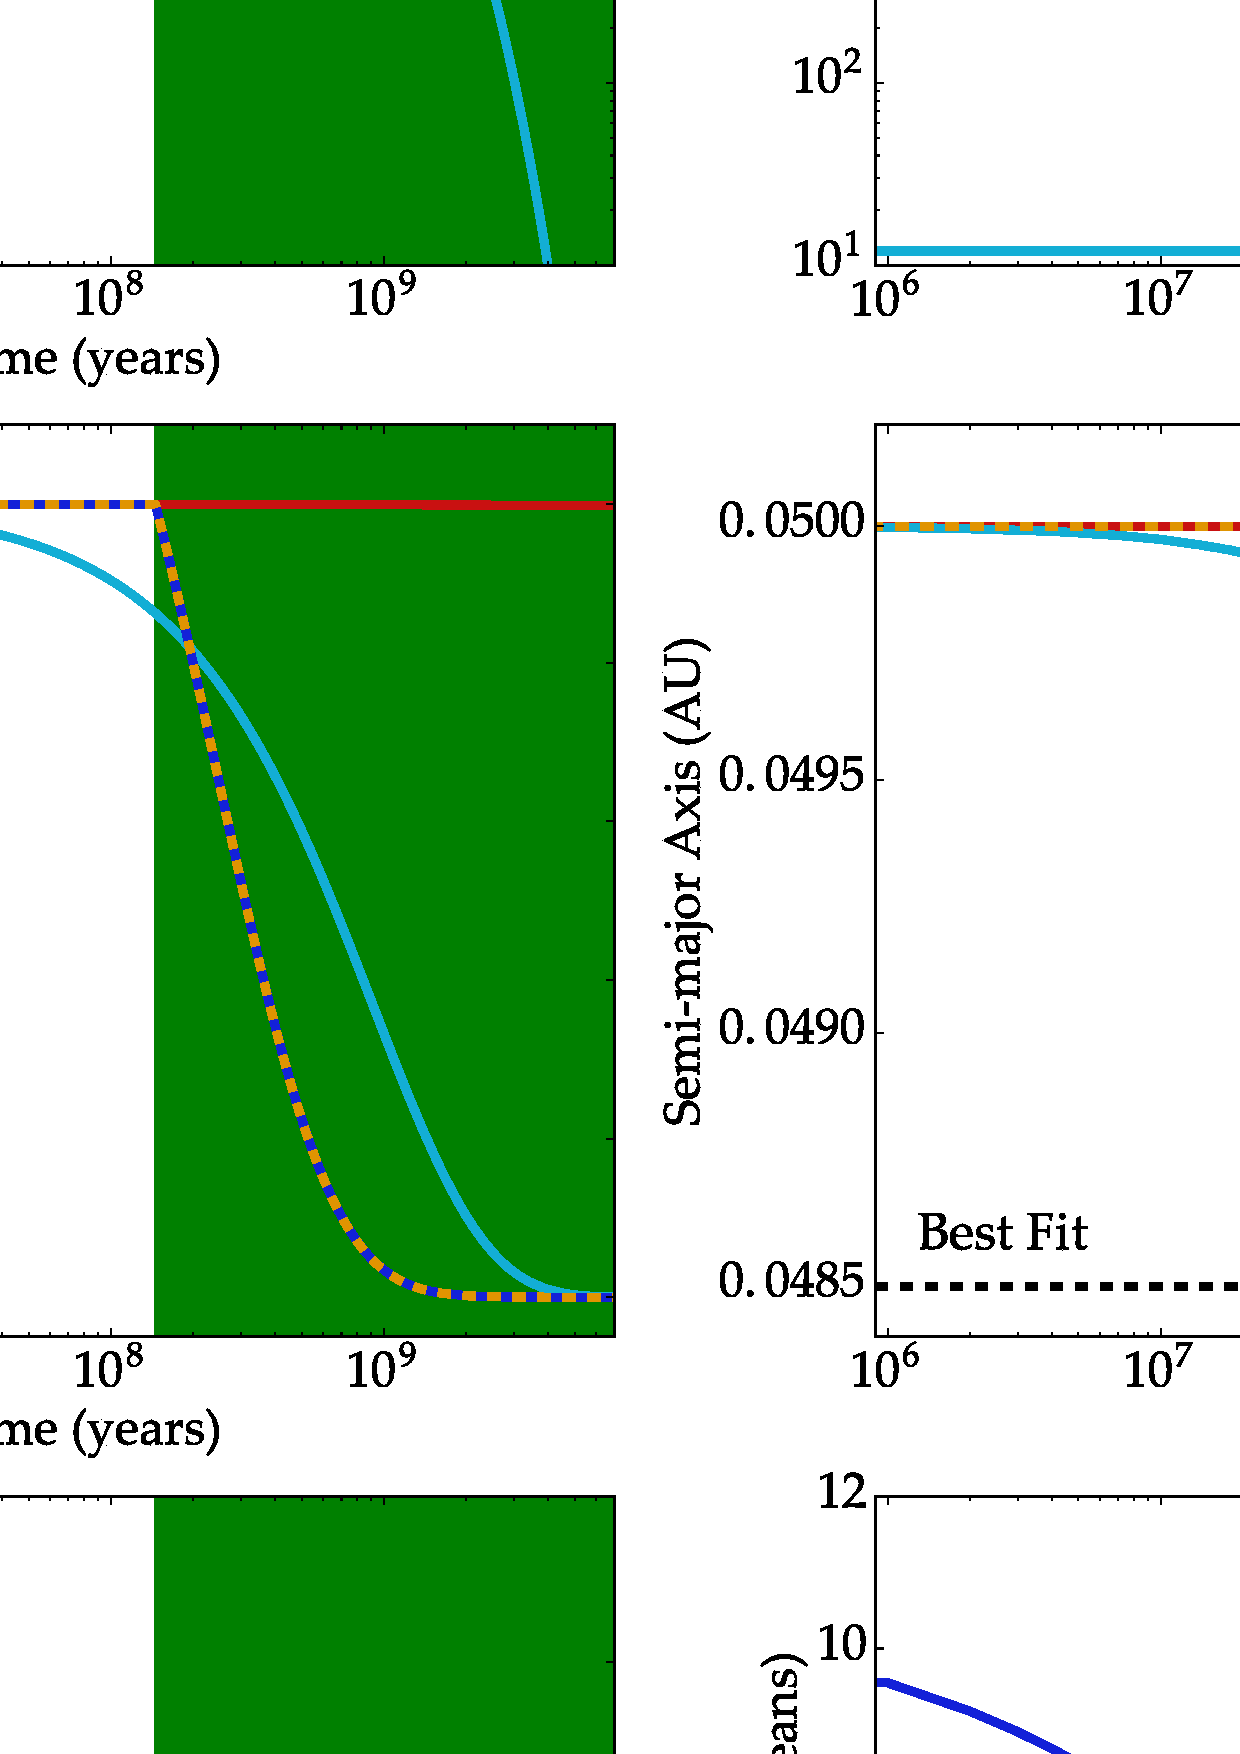
\includegraphics[width=0.75\textwidth]{tidal_hec.pdf}
\end{center}
\caption{Caption here.}
\label{fig:tidal_hec}
\end{figure}

% Fig 11: Same as 10, but c) include TidePower
% Fig 12: Same as 10, but with lines comparing oceanq, no ocean, CPL

\subsubsection{Magnetic Fields}

% Fig 13: a) MagMom, b) WindPres, c) MagRad
%       - one set of curves w/tidal heat, one w/o

\subsection{Atmospheric Evolution}
% Rodrigo

In Fig.~\ref{fig:HZEvol} we plot the evolution of the conservative HZ limits of \cite{Kopparapu13} as a function of time for a model of Proxima Centauri. The blue region is the HZ, which slowly moves inwards for 500 Myr, reaching the current orbit of Proxima b after about 200 Myr.

\begin{figure} 
\begin{center}
\includegraphics[width=0.75\textwidth]{HZEvol.ps}
\end{center}
\caption{Evolution of the conservative HZ of Proxima Centauri, along with the orbits of Proxima Centauri b (solid line) and Mercury (dashed line).}
\label{fig:HZEvol}
\end{figure}




% Fig. 14: a) water content, b) oxygen content
% Fig. 15: HEC plots: a) habitable example, b) envelope decreases, but remains, c) envelope lost, then water lost
% Fig 16: Reservoirs of water with time

\section{Discussion\label{sec:disc}}
% All

In the previous section we outlined numerous possibilities for the history of Proxima b. We considered processes spanning the planet's core to the Milky Way galaxy and find that effects at all these scales could be important in the history of our closest exoplanet. In this section, we summarize the results in terms of the potential atmospheres that Proxima b might have, and which aree considered in detail in \citep{Meadows16}. Then we examine the likelihood that it is current
ly habitable.

\subsection{Atmospheric States}

\subsubsection{Earth-Like}

We find that some scenarios allow for the planet to currently support
surface water. In particular, the ``habitable evaporated core''
\citep{Luger15} is particularly promising as it can avoid both the
high-luminosity pre-main sequence phase and any devastating tidal
heating that may occur while the planet ``surfs'' the HZ migration, or
during circularization after orbital destabilization. Such a world may
be enriched in deuterium that remained during hydrogren escape, and it
may also be geothermally active if it is young and enriched in
potassium.

Another possibility is that Proxima b formed at a larger orbital
distance and was scattered in to its current location by a system-wide
instability, which may have been triggered by a close passage with
\acen~A and B, see $\S$~\ref{sec:results}.1. If the instability
happened after the star reached the main sequence, then the planet
would have arrived in the HZ after its position had stabilized. If b's
eccentricity after the instability was larger than about 0.35, then
there is some danger that tidal heating could have triggered a runaway
greenohuse, see Fig.~\ref{fig:eqtide}, but it may have been
short-lived enough to permit habitability.

Another low-probability possibility is that even if the planet became
desiccated during the pre-MS phase, impact from water-rich bodies
could simultaneously blow off the CO$_2$ and/or $O_2$ atmosphere while
delivering water. This scenario would require fine-tuning, but we note
that close passage between Proxima and \acen~A and B could destabilize
any putative ``exo-Oort Clouds'' that could have existed around the
stars. Current numerical models do not permit a robust calculation of
this possibility, so it remains a viable path for Proxima b to be
habitable.

Although these atmospheric states permit habitability, we must bear in
mind that the rotation period is either synchronous or in a spin-orbit
resonance due to tidal effects. The rotation rate is therefore longer
than on Earth and so atmospheric dynamics would be different. If
synchronous, it would be likely that the planet's daylit side would be
covered in clouds \citep{Yang13}.

\subsubsection{Venus-Like}

Regardless of whether Prxoima b spent signficant time in a runaway
greenhouse prior to the arrival of the HZ, it could be in a runaway
greenhouse state like Venus. If it formed {\it in situ}, then this
possibility is more likely because its first $\sim$100 Myr were spent
interior to the HZand hence it may have developed a dense CO$_2$
atmosphere as has occurred on Venus. In this case, the planet is
uninhabitable as the surface temperature is too hot for liquid water,
and the higher surface temperature results from greenhouse warming by
CO$_2$.

Even if the planet avoided desiccation during the PMS stage, it is
reasonable to assume that a Venus-like atmosphere is possible. CO$_2$
is a very abundant molecule in planetary atmospheres, and given its
strong ability to heat surface, high molecular weight, and strong
chemical bonds, it may be able to accumulate in the HZ to large enough
levels to trigger the runaway greenhouse.

A final possibility, mentioned above, is that past tidal heating drove
the planet into a runaway greenhouse \citep{Barnes13}. If the planet
was ever in a high eccentricity state ($e~>~0.35$) then the surface
energy flux from the interior could have reached the critical limit of
$\sim$300 W/m$^2$ \citep{Kasting93,Abe93,Goldblatt15}. Such high
surface fluxes may be short-lived if the heating can only come from
the ocean \citep{DriscollBarnes15}.

\subsubsection{Neptune-Like}

Proxima b may have formed with sufficient hydrogen that it has
retained despite all the high energy processes that have likely
affected it. This possibility is especially likely if it formed beyond
the snowline, perhaps with 10 times more mass than it has now, and
migrated in. Even if just 1 Earth-mass, some of that may be in
hydrogen that was accreted in a much colder environment.

\subsubsection{Abiotic Oxygen Atmosphere}

If Proxima b formed with a large water inventory, the pre-MS phase may
have photolyzed water vapor and the hydrogen escaped. Although oxygen
is highly reactive, thousands of bars of oxygen can be liberated
through this mechanism \citep{LugerBarnes15} and hence all sinks for
it may become saturated \citep{Schaefer16}. In principle, thousands of
bars of oxygen could remain, but most likely it would be far
lower. This planet is unlikely to be habitable, as the oxygen builds
up early on, and large amounts of free oxygen are likely to stifle the
pre-biotic chemistry necessary for life to originate.

If the greenhouse gases are at low enough levels in the atmosphere,
then it may be possible for liquid water to accumulate on the
planetary surface and this planet would meet the traditional
definition of ``habitable.'' However, we think it would be unlikely
that life could arise on such a planet because the oxygen would
prevent the growth of the pre-biotic molecules that were necessary for
life on Earth to emerge (REF), which occured in very low oxygen
levels. Thus, the detection of atmospheric oxygen as well as the
presence of surface liquid by other means, \eg glint
\citep{Robinson10}, would not be sufficient evidence that the planet
is habitable.

\subsubsection{Abiotic Oxygen + Water Atmosphere}

If Proxima b experienced a PMS greenhouse that destroyed most, but not
all, of the water, then it is possible that the atmosphere has large
concentrations of oxygen and water. The O$_2$, H$_2$O and CO$_2$
greenhouse warming could be sufficient to prevent water from
accumulating on the surface, and hence it could have significant
abundance in the stratosphere. While the simultaneous detection of
water and oxygen has traditionally been envisaged as an ideal
combination for life-detection (REF), in the case of Proxima b, it is
insufficient to prove habitable conditions exist, let alone that life
is present.

\subsubsection{No Atmosphere}

Since Proxima b is subjected to repeated flaring events and other
activity \citep{Walker81,Davenport16}, it may be that the
atmosphere has been permanentaly destroyed. Such a process is
difficult to envision, as it would require all the volatiles in the
mantle to have been degassed and blown away. However, if the planet
was tidally heated for a long time, mantle convection may have been
vigorous and perhaps total volatile depletion is possible, especially
if the planet is of order 7 Gyr old and if the core has solidifed,
quenching the magnetic dynamo. Another possibility is that a recent
stellar eruption has temporarily stripped away the atmosphere, which
will reform by outgassing.

\subsection{Is Proxima b Habitable?}

Planetary habitability is a complicated feature to model
quantitatively and Proxima b is no different. We do know that the
planet has sufficient energy to support life, assuredly has enough
bioessential elements, and is old enough for life to have gained a
foothold, assuming Earth isn't an extreme outlier. The biggest
questions are if it is terrestrial, and if it possesses vast resevoirs
of liquid water. At this time, it is impossible to determine the
probability that it does support liquid water, so we cannot answer the
eponymous questions. As always, more data are needed.

However, our analysis does provide some important information on where
to focus future efforts. As liquid water is vital, it is paramount to
determine the pathways that allow the planet to have accreted and
retained the water. However, even if the planet forms with water, our
investigations have shown that it will not necessarily be retained. If
it formed {\it in situ} or arrived in the HZ at the time of the
dispersal of the gas disk, then Proxima b had to endure at least 100
Myr in a runaway greenhouse state, see $\S$~\ref{sec:results}.2 and
\citep{LugerBarnes15}.

Even if the planet arrived in its orbit late, perhaps following an
orbital instability, the water may have to survive a ``tidal
greenhouse'' in which tidal heating drives water loss, see
$\S$~\ref{sec:results}.3 and \citep{Barnes13}. Such high tidal heating
rates may require very large eccentricity and/or abnormally low $Q$
values, but the latter is certianly possible during planet-planet
scattering events \citep{Chatterjee08}, or perhaps by Kozai-like
oscillation driven by perturbations from the \acen~A and B pair if the
orbit of Proxima Centauri was much smaller in the past
\citep{DesideraBarbieri07}. If the additional planet in the system is
massive, on an eccentric orbit, and/or on a highly inclined orbit,
then it, too, may induce eccentricity perturbations that maintain
eccentricities \cite{TakedaRasio05}, possibly in the range of a tidal
greenhouse. As shown in $\S$~\ref{sec:results}.4, the eccentricity of
b will damp, but the timescale can be very long. Large eccentricities
are not well-modeled by equilibrium tide theory, even with a proper
accounting of geophysical features as in the \thermint module, so it
is difficult at present to assess the role of tidal heating in water
retention.

Another possible route to water loss is through temporary or permanent
atmosphere erosion by flares and coronal mass ejections. It is
possible that these events could blast away the atmosphere completely,
in which case liquid water on the surface is not stable. Should the
atmosphere reform, the water may return to the liquid state, but it is
certainly plausible that some events are powerful enough to remove the
water in one event, or, more likely, repeated bombardments would
slowly remove the atmopshere. Our analysis doesn't provide a direct
measurement of this phenomenon, but we note that some geophysical
models for the planet predict core solidification times less than the
age of the system. In those cases, the magnetic field is quenched and
is not capable of deflecting charged particles. However, it is not
clear that a magnetic field is always beneficial for life, as it also
increases the cross-sectional area of the planet for charged particles
and funnels the energy into the magnetic poles, possibly increasing
mass loss.

These processes are all clear dangers for the habitability of Proxima
b. Yet, we are also able to identify pathways that produce decidedly
Earth-like versions of planet b. As shown in Fig.~\ref{fig:qchoice},
if the planet formed with 0.1\% of its mass in a hydrogen envelope, 7
Earth oceans of water, then the combined effects of the stellar
evolution, envelope evolution and atmospheric escape, tidal evolution,
and geophysical evolution predict a planet with 1 Earth ocean of
surface water, no hydrogen envelope, and a semi-major axis within the
observed uncertainties. A planet like this could evolve similarly to
Earth, and therefore may have Earth-like conditions today.

A final possibility is that Proxima b, receiving only 65\% of Earth's
insolation, may have an ice-covered surface, but with a liquid water
mantle, similar to Europa. For such a planet, the water is heated by
the energy from accretion, radiogenic sources and/or tidal
heating. Ice is much more absorptive at the longer wavelengths of
light that Proxima emits and so it may be difficult to ice over the
planet \citep{Joshi12,Shields13}, especially since it probably spent
hundreds of Myr in a runaway greenhouse. But if a reflective haze
and/or cloud layer could form, it could reflect away the light before
it reaches the surface. This possibility seems unlikely, but we cannot
rule out that the planet is a ``super-Europa'' \citep{BarnesHeller13},
a scaled up version of the icy satellites of our Solar System and with
a potentially inhabited subsurface water layer.

So Proxima b may or may not be habitable. While we are only able to
identify a narrow range of pathways that permit habitability, we must
bear in mind that our model, while including phenomena over sizescales
of meters to kpc, is simple and does not include many potential
feedbacks. The geochemistry of exoplanets is a gaping hole in
scientific knowledge, and one can easily imagine how other systems may
maintain liquid water with geochemical cycles not present in our Solar
System. Similarly, liquid surface water may represent a sort of
``planetary attractor'', in which planets in the HZ naturally and
typically evolve toward a state in which their surfaces support liquid
water.

\section{Conclusions\label{sec:concl}}
% Rory
We have performed a comprehensive analysis of the evolution of the
Alpha Centauri triple star system with a specific focus on Proxima Centauri b's
habitability. We find that many disparate factors are important,
including from the stellar system's orbit in the galaxy
($\S$~\ref{sec:results}.1), the orbital and rotational evolution of
the planets ($\S$~\ref{sec:results}.2), the stellar evolution
($\S$~\ref{sec:results}.3), geophysical evolution
($\S$~\ref{sec:results}.4), and atmospheric evolution
($\S$~\ref{sec:results}.5). We find that many evolutionary pathways
are admitted by the data and hence the planet may currently exist in
many possible states.

We conclude that Proxima b may be habitable, but identify the
retention of water as the biggest obstacle for Proxima b to support
life. Water loss may occur through multiple channels operating in
tandem or in isolation, including desiccation during the Pre-MS,
excessive tidal heating, or atmospheric destruction by flares and
coronal mass ejections. We find the most likely pathway for
habitability is if planet b formed with a thin hydrogen envelope of
order $10^{-3}~\mearth$ which was eroded by the early XUV evolution of
the host star, see $\S$~\ref{sec:results}.3 and \citep{Luger15}. In
that case, Proxima b is a ``habitable evaporated core'' and has
followed a very different trajectory than Earth did on their paths to
liquid surface water.

Regardless of Proxima's habitability, it offers scientists an
unprecendented window into the nature of terrestrial planets. At only
1.3 pc distance, we will be able to study this planet in detail with
future missions, should they be designed appropriately, see
\citep{Meadows16}. If Proxima b is uninhabitable, we may be able to
determine how that happened and how Earth avoided the same fate. At a
minimum, the discovery of Proxima Centauri b has ushered in a new era
in comparative planetology, or perhaps it is the first step in the
discovery of extraterrestrial life.
 
\vspace{1cm}
This work was supported by the NASA Astrobiology Institute's Virtual
Planetary Laboratory under Cooperative Agreement number NNA13AA93A.
David Fleming is supported by an NSF IGERT DGE-1258485 fellowship.


\bibliography{bib}

\end{document}  
